\documentclass[%
	fontsize=11pt,% bigger font
	paper=a4,% paper size
	pagesize,% set pagesize in PDF
	twoside=false,% =oneside
	listof=totoc,%add list of figures to toc
	draft% TODO remove this!
]{scrbook}

%---------------------------------------
%---------PACKAGES----------------------
%---------------------------------------

% language
\usepackage[english]{babel}

% font config
\usepackage{libertine}
\usepackage[T1]{fontenc}

% microtype
\usepackage[activate={true,nocompatibility},final,tracking=true,kerning=true,spacing=nonfrench,factor=1100,stretch=10,shrink=10]{microtype}
% activate={true,nocompatibility} - activate protrusion and expansion
% final - enable microtype; use "draft" to disable
% tracking=true, kerning=true, spacing=true - activate these techniques
% factor=1100 - add 10% to the protrusion amount (default is 1000)
% stretch=10, shrink=10 - reduce stretchability/shrinkability (default is 20/20)

% links
\usepackage{hyperref}

% math
\usepackage{amsmath}

% graphics
\usepackage{tikz}
\usepackage{tikz-3dplot}

% glossar
% dep: hyperref
\usepackage[
	toc%add to toc
]{glossaries}

% TODO remove this!
% debug packages
\usepackage{blindtext}


%---------------------------------------
%---------SETTINGS----------------------
%---------------------------------------

% general informaion
\title{Some funny words}
\author{Marco Neumann}

% color
\definecolor{colcontrast}{RGB}{255,0,0}

% links
\hypersetup{
	colorlinks,% colored text instead of borders
	linkcolor=black,% black inter document links
	urlcolor=black,% black urls
	final% also work in draft mode, TODO remove this!
}

% tikz
\usetikzlibrary{arrows}
\tikzset{
	>=stealth',
	axis/.style={->, very thick, >=stealth'}
}


%---------------------------------------
%---------GLOSSARY----------------------
%---------------------------------------

\newglossaryentry{random number generator}
{
	name={Random Number Generator},
	description={Generates random numbers}
}

\newacronym{rng}{RNG}{\glslink{random number generator}{Random Number Generator}}

\makeglossaries% build glossary
\glsunsetall% fix acronyms


\begin{document}

\frontmatter
\maketitle
\tableofcontents

\mainmatter
\chapter{How to beat the system}
The method described in this thesis has some weaknesses. I will construct a dateset, which is not processed very well and I will discuss, why this type of data is not very common.

\section{Constructing a special dataset}
Consider the following a dataset, that is made of many random points $(x, y, z) \in \left[0, 1\right)^3$, that satisfy the following constraint:
\begin{equation}\label{eq:beat}
	(x + y + z) \bmod 1 = 0
\end{equation}
The points are uniform distributed if you project them on one or two dimensions. But if you calculate the three dimensional distribution, the points do not show a uniform distribution. (see Figure~\ref{fig:beat}). Because the generated points have two degrees of freedom, the two dimensional distribution test will fail. It is also possible to generate datasets with even more degrees of freedom using the same technique.\footnote{You may not be able to imagine datasets with more than three dimensions. For 4 dimensions, you find some help: \url{http://crepererum.github.io/brain4D/\#constructed.csv}}
\begin{figure}
	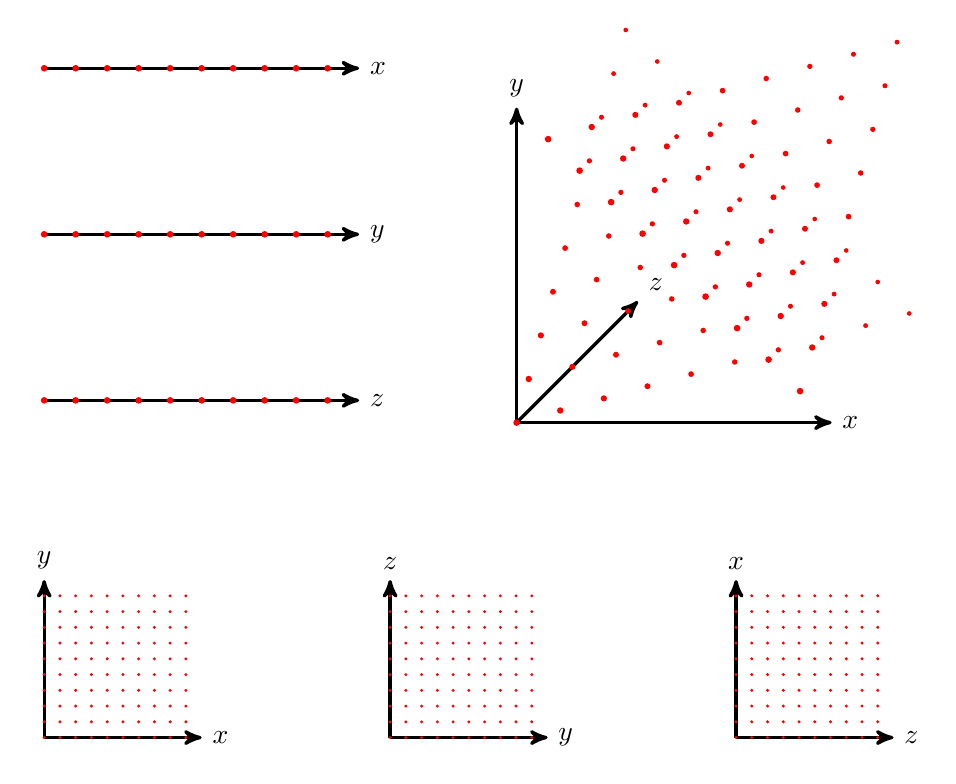
\begin{tikzpicture}[scale = 5.0]
	\begin{scope}
		\foreach \name [count=\d from 0] in {x,y,z} {
			\begin{scope}[yshift=-\d*12]
				\begin{scope}[scale=0.8]
					\draw[axis] (0,0) -- (1,0) node[right]{$\name$};
					\foreach \x in {0,...,9} {
						\fill[colcontrast] (\x/10,0) circle(0.3pt);
					}
				\end{scope}
			\end{scope}
		}
	\end{scope}
	\begin{scope}[shift={(0,-1.7)}]
		\foreach \namefirst/\namesecond [count=\d from 0] in {x/y,y/z,z/x} {
			\begin{scope}[xshift=\d*25]
				\begin{scope}[scale=0.4]
					\draw[axis] (0,0) -- (1,0) node[right]{$\namefirst$};
					\draw[axis] (0,0) -- (0,1) node[above]{$\namesecond$};
					\foreach \x in {0,...,9} {
						\foreach \y in {0,...,9} {
							\fill[colcontrast] (\x/10,\y/10) circle(0.3pt);
						}
					}
				\end{scope}
			\end{scope}
		}
	\end{scope}
	\begin{scope}[shift={(1.2,-0.9)}]
		\begin{scope}[scale=0.8]
			\draw[axis] (0,0,0) -- (1,0,0) node[right]{$x$};
			\draw[axis] (0,0,0) -- (0,1,0) node[above]{$y$};
			\draw[axis] (0,0,0) -- (0,0,-1) node[above right]{$z$};
			\foreach \x in {0,...,9} {
				\foreach \y in {0,...,9} {
					\pgfmathsetmacro{\z}{mod(\x+\y,10)}
					\fill[colcontrast] (\x/10,\y/10,-\z/10) circle(0.3pt-0.1pt*\z/10);
				}
			}
		\end{scope}
	\end{scope}
\end{tikzpicture}


	\caption{Situation described in Equation~\ref{eq:beat}}
	\label{fig:beat}
\end{figure}

\appendix

\backmatter
\listoffigures
\printglossaries

\end{document}

